\section{Sp\-Tuple.h File Reference}
\label{SpTuple_8h}\index{SpTuple.h@{SpTuple.h}}
{\tt \#include \char`\"{}Sp\-Maths.h\char`\"{}}\par
{\tt \#include $<$memory$>$}\par
{\tt \#include $<$cassert$>$}\par
{\tt \#include \char`\"{}Sp\-Tuple.inc\char`\"{}}\par


Include dependency graph for Sp\-Tuple.h:\begin{figure}[H]
\begin{center}
\leavevmode
\includegraphics[width=176pt]{SpTuple_8h__incl}
\end{center}
\end{figure}


This graph shows which files directly or indirectly include this file:\begin{figure}[H]
\begin{center}
\leavevmode
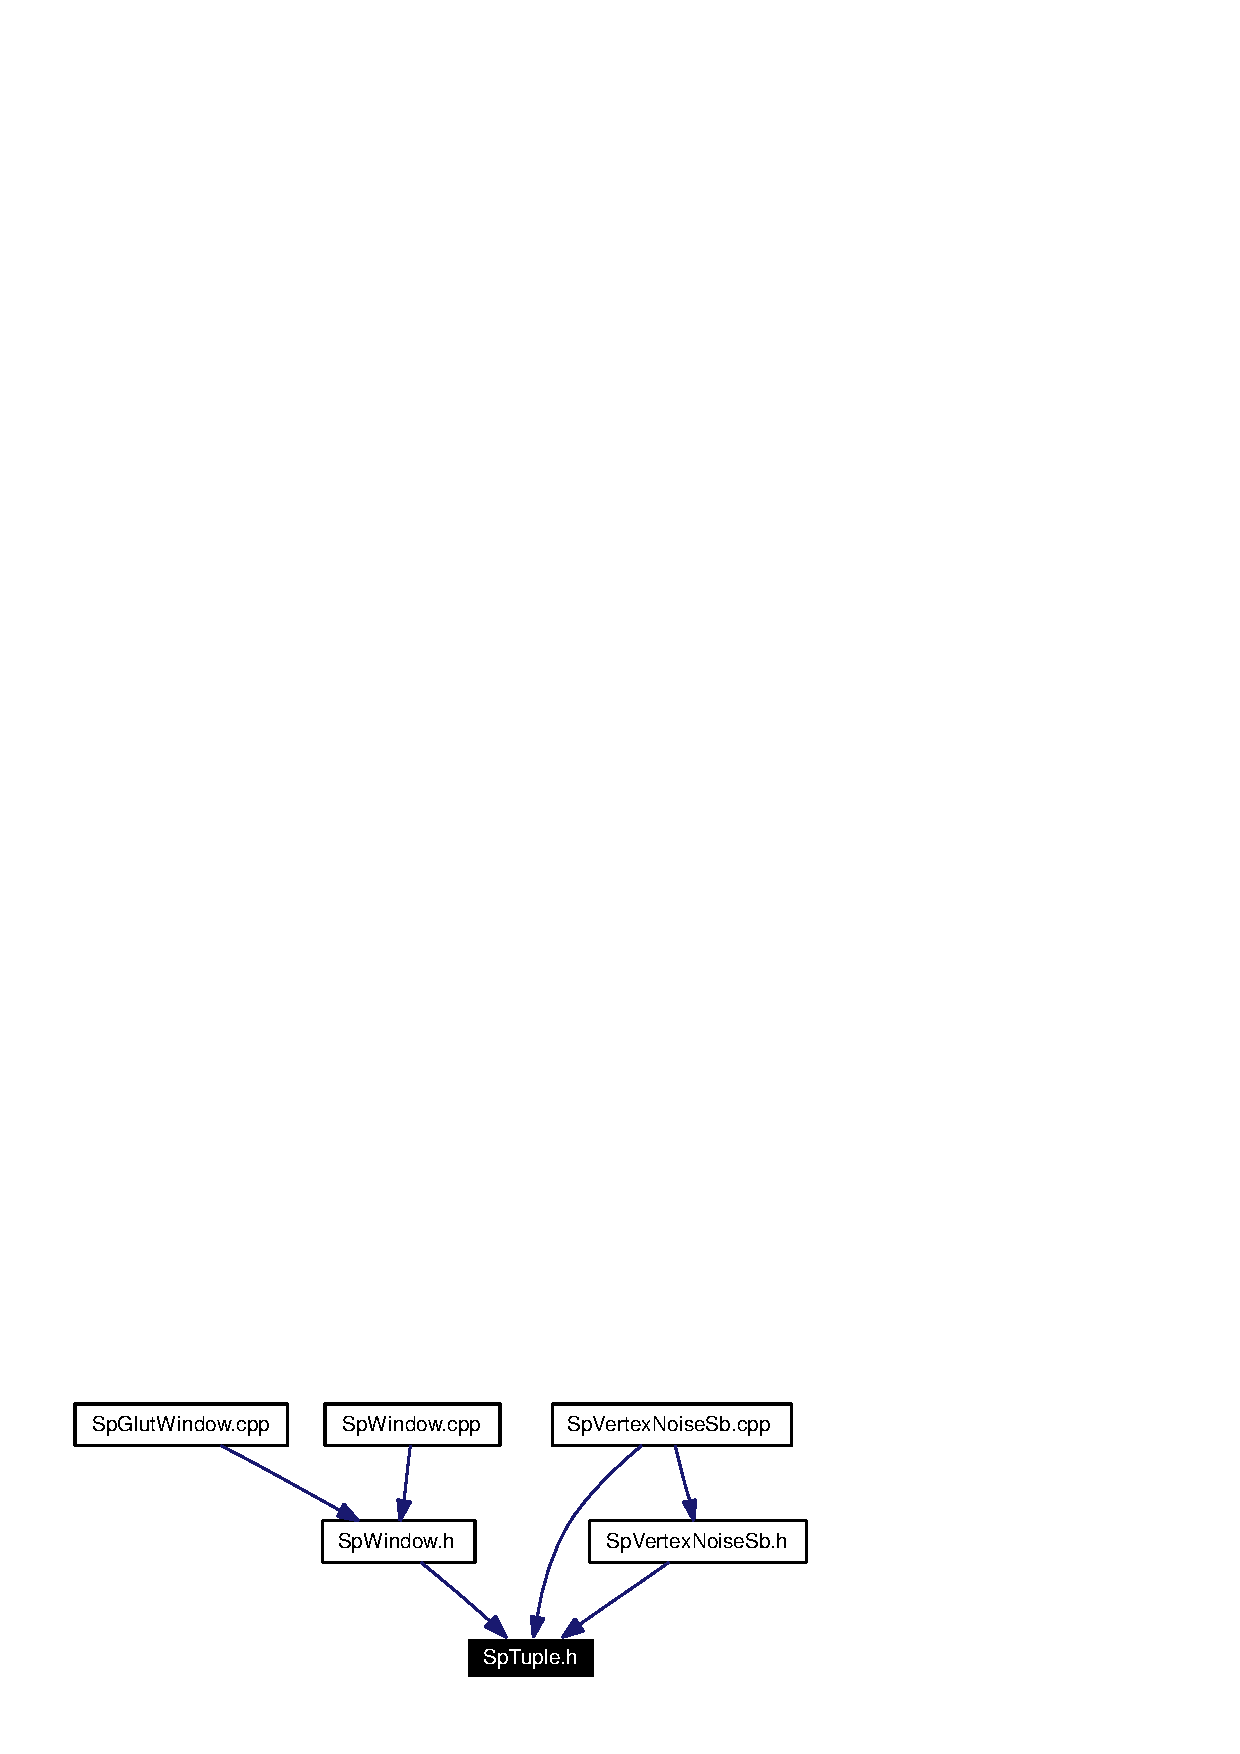
\includegraphics[width=194pt]{SpTuple_8h__dep__incl}
\end{center}
\end{figure}
\subsection*{Namespaces}
\begin{CompactItemize}
\item 
namespace {\bf Spark}
\end{CompactItemize}
\subsection*{Classes}
\begin{CompactItemize}
\item 
class {\bf Spark::Sp\-Tuple$<$ N, Real $>$}
\begin{CompactList}\small\item\em N-Dimensional data class with support for vector mathematics. \item\end{CompactList}\item 
class {\bf Spark::Sp\-Tuple2$<$ Real $>$}
\begin{CompactList}\small\item\em 2D tuple data class with support for vector mathematics \item\end{CompactList}\item 
class {\bf Spark::Sp\-Tuple3$<$ Real $>$}
\begin{CompactList}\small\item\em 3D tuple data class with support for vector mathematics \item\end{CompactList}\item 
class {\bf Spark::Sp\-Tuple4$<$ Real $>$}
\begin{CompactList}\small\item\em 4D tuple data class with support for vector mathematics \item\end{CompactList}\end{CompactItemize}
\subsection*{Typedefs}
\begin{CompactItemize}
\item 
typedef Sp\-Tuple2$<$ float $>$ {\bf vec2}
\item 
typedef Sp\-Tuple3$<$ float $>$ {\bf vec3}
\item 
typedef Sp\-Tuple4$<$ float $>$ {\bf vec4}
\item 
typedef Sp\-Tuple2$<$ int $>$ {\bf ivec2}
\item 
typedef Sp\-Tuple3$<$ int $>$ {\bf ivec3}
\item 
typedef Sp\-Tuple4$<$ int $>$ {\bf ivec4}
\item 
typedef Sp\-Tuple2$<$ bool $>$ {\bf bvec2}
\item 
typedef Sp\-Tuple3$<$ bool $>$ {\bf bvec3}
\item 
typedef Sp\-Tuple4$<$ bool $>$ {\bf bvec4}
\item 
typedef Sp\-Tuple2$<$ float $>$ {\bf float2}
\item 
typedef Sp\-Tuple3$<$ float $>$ {\bf float3}
\item 
typedef Sp\-Tuple4$<$ float $>$ {\bf float4}
\item 
typedef Sp\-Tuple2$<$ float $>$ {\bf Sp\-Vector2f}
\item 
typedef Sp\-Tuple3$<$ float $>$ {\bf Sp\-Vector3f}
\item 
typedef Sp\-Tuple4$<$ float $>$ {\bf Sp\-Vector4f}
\item 
typedef Sp\-Tuple3$<$ char $>$ {\bf Sp\-Color3b}
\item 
typedef Sp\-Tuple4$<$ char $>$ {\bf Sp\-Color4b}
\item 
typedef Sp\-Tuple3$<$ unsigned char $>$ {\bf Sp\-Color3ub}
\item 
typedef Sp\-Tuple4$<$ unsigned char $>$ {\bf Sp\-Color4ub}
\item 
typedef Sp\-Tuple3$<$ int $>$ {\bf Sp\-Color3i}
\item 
typedef Sp\-Tuple4$<$ int $>$ {\bf Sp\-Color4i}
\item 
typedef Sp\-Tuple3$<$ unsigned int $>$ {\bf Sp\-Color3ui}
\item 
typedef Sp\-Tuple4$<$ unsigned int $>$ {\bf Sp\-Color4ui}
\item 
typedef Sp\-Tuple3$<$ float $>$ {\bf Sp\-Color3f}
\item 
typedef Sp\-Tuple4$<$ float $>$ {\bf Sp\-Color4f}
\end{CompactItemize}
\subsection*{Functions}
\begin{CompactItemize}
\item 
template$<$unsigned int N, class Real$>$ Sp\-Tuple$<$ N, Real $>$ {\bf operator $\ast$} (Real f\-Scalar, const Sp\-Tuple$<$ N, Real $>$ \&rk\-V)
\item 
template$<$unsigned int N, class Real$>$ Real {\bf Length} (const Sp\-Tuple$<$ N, Real $>$ \&rk\-V)
\item 
template$<$unsigned int N, class Real$>$ Real {\bf Length\-Squared} (const Sp\-Tuple$<$ N, Real $>$ \&rk\-V)
\item 
template$<$unsigned int N, class Real$>$ Real {\bf Dot} (const Sp\-Tuple$<$ N, Real $>$ \&rk\-A, const Sp\-Tuple$<$ N, Real $>$ \&rk\-B)
\item 
template$<$unsigned int N, class Real$>$ Sp\-Tuple$<$ N, Real $>$ {\bf Normalize} (const Sp\-Tuple$<$ N, Real $>$ \&rk\-V)
\item 
template$<$unsigned int N, class Real$>$ Sp\-Tuple$<$ N, Real $>$ {\bf Clamp} (const Sp\-Tuple$<$ N, Real $>$ \&rk\-V, Real f\-Min, Real f\-Max)
\item 
template$<$unsigned int N, class Real$>$ Sp\-Tuple$<$ N, Real $>$ {\bf Offset} (const Sp\-Tuple$<$ N, Real $>$ \&rk\-V, Real f\-Offset)
\item 
template$<$class Real$>$ Sp\-Tuple3$<$ Real $>$ {\bf Normalize} (const Sp\-Tuple3$<$ Real $>$ \&rk\-V)
\item 
template$<$class Real$>$ Sp\-Tuple3$<$ Real $>$ {\bf Normalized\-Cross} (const Sp\-Tuple3$<$ Real $>$ \&rk\-V1, const Sp\-Tuple3$<$ Real $>$ \&rk\-V2)
\item 
template$<$class Real$>$ Sp\-Tuple3$<$ Real $>$ {\bf Cross} (const Sp\-Tuple3$<$ Real $>$ \&rk\-V1, const Sp\-Tuple3$<$ Real $>$ \&rk\-V2)
\item 
template$<$class Real$>$ Sp\-Tuple4$<$ Real $>$ {\bf Normalize} (const Sp\-Tuple4$<$ Real $>$ \&rk\-V)
\item 
template$<$class Real$>$ Sp\-Tuple4$<$ Real $>$ {\bf Normalized\-Cross} (const Sp\-Tuple4$<$ Real $>$ \&rk\-V1, const Sp\-Tuple4$<$ Real $>$ \&rk\-V2)
\item 
template$<$class Real$>$ Sp\-Tuple4$<$ Real $>$ {\bf Cross} (const Sp\-Tuple4$<$ Real $>$ \&rk\-V1, const Sp\-Tuple4$<$ Real $>$ \&rk\-V2)
\end{CompactItemize}


\subsection{Typedef Documentation}
\index{SpTuple.h@{Sp\-Tuple.h}!bvec2@{bvec2}}
\index{bvec2@{bvec2}!SpTuple.h@{Sp\-Tuple.h}}
\subsubsection{\setlength{\rightskip}{0pt plus 5cm}typedef Sp\-Tuple2$<$bool$>$ {\bf Spark::bvec2}}\label{namespaceSpark_a13}


Definition at line 715 of file Sp\-Tuple.h.

Referenced by Spark::Sp\-Tuple$<$ N, Real $>$::Sp\-Tuple().\index{SpTuple.h@{Sp\-Tuple.h}!bvec3@{bvec3}}
\index{bvec3@{bvec3}!SpTuple.h@{Sp\-Tuple.h}}
\subsubsection{\setlength{\rightskip}{0pt plus 5cm}typedef Sp\-Tuple3$<$bool$>$ {\bf Spark::bvec3}}\label{namespaceSpark_a14}


Definition at line 716 of file Sp\-Tuple.h.

Referenced by Spark::Sp\-Tuple$<$ N, Real $>$::Sp\-Tuple().\index{SpTuple.h@{Sp\-Tuple.h}!bvec4@{bvec4}}
\index{bvec4@{bvec4}!SpTuple.h@{Sp\-Tuple.h}}
\subsubsection{\setlength{\rightskip}{0pt plus 5cm}typedef Sp\-Tuple4$<$bool$>$ {\bf Spark::bvec4}}\label{namespaceSpark_a15}


Definition at line 717 of file Sp\-Tuple.h.

Referenced by Spark::Sp\-Tuple$<$ N, Real $>$::Sp\-Tuple().\index{SpTuple.h@{Sp\-Tuple.h}!float2@{float2}}
\index{float2@{float2}!SpTuple.h@{Sp\-Tuple.h}}
\subsubsection{\setlength{\rightskip}{0pt plus 5cm}typedef Sp\-Tuple2$<$float$>$ {\bf Spark::float2}}\label{namespaceSpark_a16}


Definition at line 719 of file Sp\-Tuple.h.

Referenced by Spark::Sp\-Tuple$<$ N, Real $>$::Sp\-Tuple().\index{SpTuple.h@{Sp\-Tuple.h}!float3@{float3}}
\index{float3@{float3}!SpTuple.h@{Sp\-Tuple.h}}
\subsubsection{\setlength{\rightskip}{0pt plus 5cm}typedef Sp\-Tuple3$<$float$>$ {\bf Spark::float3}}\label{namespaceSpark_a17}


Definition at line 720 of file Sp\-Tuple.h.

Referenced by Spark::Sp\-Tuple$<$ N, Real $>$::Sp\-Tuple().\index{SpTuple.h@{Sp\-Tuple.h}!float4@{float4}}
\index{float4@{float4}!SpTuple.h@{Sp\-Tuple.h}}
\subsubsection{\setlength{\rightskip}{0pt plus 5cm}typedef Sp\-Tuple4$<$float$>$ {\bf Spark::float4}}\label{namespaceSpark_a18}


Definition at line 721 of file Sp\-Tuple.h.

Referenced by Spark::Sp\-Tuple$<$ N, Real $>$::Sp\-Tuple().\index{SpTuple.h@{Sp\-Tuple.h}!ivec2@{ivec2}}
\index{ivec2@{ivec2}!SpTuple.h@{Sp\-Tuple.h}}
\subsubsection{\setlength{\rightskip}{0pt plus 5cm}typedef Sp\-Tuple2$<$int$>$ {\bf Spark::ivec2}}\label{namespaceSpark_a10}


Definition at line 711 of file Sp\-Tuple.h.

Referenced by Spark::Sp\-Tuple$<$ N, Real $>$::Sp\-Tuple().\index{SpTuple.h@{Sp\-Tuple.h}!ivec3@{ivec3}}
\index{ivec3@{ivec3}!SpTuple.h@{Sp\-Tuple.h}}
\subsubsection{\setlength{\rightskip}{0pt plus 5cm}typedef Sp\-Tuple3$<$int$>$ {\bf Spark::ivec3}}\label{namespaceSpark_a11}


Definition at line 712 of file Sp\-Tuple.h.

Referenced by Spark::Sp\-Tuple$<$ N, Real $>$::Sp\-Tuple().\index{SpTuple.h@{Sp\-Tuple.h}!ivec4@{ivec4}}
\index{ivec4@{ivec4}!SpTuple.h@{Sp\-Tuple.h}}
\subsubsection{\setlength{\rightskip}{0pt plus 5cm}typedef Sp\-Tuple4$<$int$>$ {\bf Spark::ivec4}}\label{namespaceSpark_a12}


Definition at line 713 of file Sp\-Tuple.h.

Referenced by Spark::Sp\-Tuple$<$ N, Real $>$::Sp\-Tuple().\index{SpTuple.h@{Sp\-Tuple.h}!SpColor3b@{SpColor3b}}
\index{SpColor3b@{SpColor3b}!SpTuple.h@{Sp\-Tuple.h}}
\subsubsection{\setlength{\rightskip}{0pt plus 5cm}typedef Sp\-Tuple3$<$char$>$ {\bf Spark::Sp\-Color3b}}\label{namespaceSpark_a22}


Definition at line 727 of file Sp\-Tuple.h.

Referenced by Spark::Sp\-Tuple$<$ N, Real $>$::Sp\-Tuple().\index{SpTuple.h@{Sp\-Tuple.h}!SpColor3f@{SpColor3f}}
\index{SpColor3f@{SpColor3f}!SpTuple.h@{Sp\-Tuple.h}}
\subsubsection{\setlength{\rightskip}{0pt plus 5cm}typedef Sp\-Tuple3$<$float$>$ {\bf Spark::Sp\-Color3f}}\label{namespaceSpark_a30}


Definition at line 739 of file Sp\-Tuple.h.

Referenced by Spark::Sp\-Tuple$<$ N, Real $>$::values().\index{SpTuple.h@{Sp\-Tuple.h}!SpColor3i@{SpColor3i}}
\index{SpColor3i@{SpColor3i}!SpTuple.h@{Sp\-Tuple.h}}
\subsubsection{\setlength{\rightskip}{0pt plus 5cm}typedef Sp\-Tuple3$<$int$>$ {\bf Spark::Sp\-Color3i}}\label{namespaceSpark_a26}


Definition at line 733 of file Sp\-Tuple.h.

Referenced by Spark::Sp\-Tuple$<$ N, Real $>$::Sp\-Tuple().\index{SpTuple.h@{Sp\-Tuple.h}!SpColor3ub@{SpColor3ub}}
\index{SpColor3ub@{SpColor3ub}!SpTuple.h@{Sp\-Tuple.h}}
\subsubsection{\setlength{\rightskip}{0pt plus 5cm}typedef Sp\-Tuple3$<$unsigned char$>$ {\bf Spark::Sp\-Color3ub}}\label{namespaceSpark_a24}


Definition at line 730 of file Sp\-Tuple.h.

Referenced by Spark::Sp\-Tuple$<$ N, Real $>$::Sp\-Tuple().\index{SpTuple.h@{Sp\-Tuple.h}!SpColor3ui@{SpColor3ui}}
\index{SpColor3ui@{SpColor3ui}!SpTuple.h@{Sp\-Tuple.h}}
\subsubsection{\setlength{\rightskip}{0pt plus 5cm}typedef Sp\-Tuple3$<$unsigned int$>$ {\bf Spark::Sp\-Color3ui}}\label{namespaceSpark_a28}


Definition at line 736 of file Sp\-Tuple.h.

Referenced by Spark::Sp\-Tuple$<$ N, Real $>$::values().\index{SpTuple.h@{Sp\-Tuple.h}!SpColor4b@{SpColor4b}}
\index{SpColor4b@{SpColor4b}!SpTuple.h@{Sp\-Tuple.h}}
\subsubsection{\setlength{\rightskip}{0pt plus 5cm}typedef Sp\-Tuple4$<$char$>$ {\bf Spark::Sp\-Color4b}}\label{namespaceSpark_a23}


Definition at line 728 of file Sp\-Tuple.h.

Referenced by Spark::Sp\-Tuple$<$ N, Real $>$::Sp\-Tuple().\index{SpTuple.h@{Sp\-Tuple.h}!SpColor4f@{SpColor4f}}
\index{SpColor4f@{SpColor4f}!SpTuple.h@{Sp\-Tuple.h}}
\subsubsection{\setlength{\rightskip}{0pt plus 5cm}typedef Sp\-Tuple4$<$float$>$ {\bf Spark::Sp\-Color4f}}\label{namespaceSpark_a31}


Definition at line 740 of file Sp\-Tuple.h.

Referenced by Spark::Sp\-Window::draw\-Frame\-Rate(), Spark::Sp\-Window::draw\-String(), Spark::Sp\-Window::Sp\-Window(), and Spark::Sp\-Tuple$<$ N, Real $>$::values().\index{SpTuple.h@{Sp\-Tuple.h}!SpColor4i@{SpColor4i}}
\index{SpColor4i@{SpColor4i}!SpTuple.h@{Sp\-Tuple.h}}
\subsubsection{\setlength{\rightskip}{0pt plus 5cm}typedef Sp\-Tuple4$<$int$>$ {\bf Spark::Sp\-Color4i}}\label{namespaceSpark_a27}


Definition at line 734 of file Sp\-Tuple.h.

Referenced by Spark::Sp\-Tuple$<$ N, Real $>$::Sp\-Tuple().\index{SpTuple.h@{Sp\-Tuple.h}!SpColor4ub@{SpColor4ub}}
\index{SpColor4ub@{SpColor4ub}!SpTuple.h@{Sp\-Tuple.h}}
\subsubsection{\setlength{\rightskip}{0pt plus 5cm}typedef Sp\-Tuple4$<$unsigned char$>$ {\bf Spark::Sp\-Color4ub}}\label{namespaceSpark_a25}


Definition at line 731 of file Sp\-Tuple.h.

Referenced by Spark::Sp\-Tuple$<$ N, Real $>$::Sp\-Tuple().\index{SpTuple.h@{Sp\-Tuple.h}!SpColor4ui@{SpColor4ui}}
\index{SpColor4ui@{SpColor4ui}!SpTuple.h@{Sp\-Tuple.h}}
\subsubsection{\setlength{\rightskip}{0pt plus 5cm}typedef Sp\-Tuple4$<$unsigned int$>$ {\bf Spark::Sp\-Color4ui}}\label{namespaceSpark_a29}


Definition at line 737 of file Sp\-Tuple.h.

Referenced by Spark::Sp\-Tuple$<$ N, Real $>$::values().\index{SpTuple.h@{Sp\-Tuple.h}!SpVector2f@{SpVector2f}}
\index{SpVector2f@{SpVector2f}!SpTuple.h@{Sp\-Tuple.h}}
\subsubsection{\setlength{\rightskip}{0pt plus 5cm}typedef Sp\-Tuple2$<$float$>$ {\bf Spark::Sp\-Vector2f}}\label{namespaceSpark_a19}


Definition at line 723 of file Sp\-Tuple.h.

Referenced by Spark::Sp\-Tuple$<$ N, Real $>$::Sp\-Tuple().\index{SpTuple.h@{Sp\-Tuple.h}!SpVector3f@{SpVector3f}}
\index{SpVector3f@{SpVector3f}!SpTuple.h@{Sp\-Tuple.h}}
\subsubsection{\setlength{\rightskip}{0pt plus 5cm}typedef Sp\-Tuple3$<$float$>$ {\bf Spark::Sp\-Vector3f}}\label{namespaceSpark_a20}


Definition at line 724 of file Sp\-Tuple.h.

Referenced by Spark::Sp\-Tuple$<$ N, Real $>$::Sp\-Tuple().\index{SpTuple.h@{Sp\-Tuple.h}!SpVector4f@{SpVector4f}}
\index{SpVector4f@{SpVector4f}!SpTuple.h@{Sp\-Tuple.h}}
\subsubsection{\setlength{\rightskip}{0pt plus 5cm}typedef Sp\-Tuple4$<$float$>$ {\bf Spark::Sp\-Vector4f}}\label{namespaceSpark_a21}


Definition at line 725 of file Sp\-Tuple.h.

Referenced by Spark::Sp\-Vertex\-Noise\-Sb::initialize(), and Spark::Sp\-Tuple$<$ N, Real $>$::Sp\-Tuple().\index{SpTuple.h@{Sp\-Tuple.h}!vec2@{vec2}}
\index{vec2@{vec2}!SpTuple.h@{Sp\-Tuple.h}}
\subsubsection{\setlength{\rightskip}{0pt plus 5cm}typedef Sp\-Tuple2$<$float$>$ {\bf Spark::vec2}}\label{namespaceSpark_a7}


Definition at line 707 of file Sp\-Tuple.h.

Referenced by Spark::Sp\-Tuple$<$ N, Real $>$::Sp\-Tuple().\index{SpTuple.h@{Sp\-Tuple.h}!vec3@{vec3}}
\index{vec3@{vec3}!SpTuple.h@{Sp\-Tuple.h}}
\subsubsection{\setlength{\rightskip}{0pt plus 5cm}typedef Sp\-Tuple3$<$float$>$ {\bf Spark::vec3}}\label{namespaceSpark_a8}


Definition at line 708 of file Sp\-Tuple.h.

Referenced by Spark::Sp\-Tuple$<$ N, Real $>$::Sp\-Tuple().\index{SpTuple.h@{Sp\-Tuple.h}!vec4@{vec4}}
\index{vec4@{vec4}!SpTuple.h@{Sp\-Tuple.h}}
\subsubsection{\setlength{\rightskip}{0pt plus 5cm}typedef Sp\-Tuple4$<$float$>$ {\bf Spark::vec4}}\label{namespaceSpark_a9}


Definition at line 709 of file Sp\-Tuple.h.

Referenced by Spark::Sp\-Tuple$<$ N, Real $>$::Sp\-Tuple().

\subsection{Function Documentation}
\index{SpTuple.h@{Sp\-Tuple.h}!Clamp@{Clamp}}
\index{Clamp@{Clamp}!SpTuple.h@{Sp\-Tuple.h}}
\subsubsection{\setlength{\rightskip}{0pt plus 5cm}template$<$unsigned int N, class Real$>$ Sp\-Tuple$<$ N, Real $>$ Spark::Clamp (const Sp\-Tuple$<$ N, Real $>$ \& {\em rk\-V}, Real {\em f\-Min}, Real {\em f\-Max})}\label{namespaceSpark_a123}


Definition at line 594 of file Sp\-Tuple.h.\index{SpTuple.h@{Sp\-Tuple.h}!Cross@{Cross}}
\index{Cross@{Cross}!SpTuple.h@{Sp\-Tuple.h}}
\subsubsection{\setlength{\rightskip}{0pt plus 5cm}template$<$class Real$>$ Sp\-Tuple4$<$ Real $>$ Spark::Cross (const Sp\-Tuple4$<$ Real $>$ \& {\em rk\-V1}, const Sp\-Tuple4$<$ Real $>$ \& {\em rk\-V2})}\label{namespaceSpark_a130}


Definition at line 692 of file Sp\-Tuple.h.\index{SpTuple.h@{Sp\-Tuple.h}!Cross@{Cross}}
\index{Cross@{Cross}!SpTuple.h@{Sp\-Tuple.h}}
\subsubsection{\setlength{\rightskip}{0pt plus 5cm}template$<$class Real$>$ Sp\-Tuple3$<$ Real $>$ Spark::Cross (const Sp\-Tuple3$<$ Real $>$ \& {\em rk\-V1}, const Sp\-Tuple3$<$ Real $>$ \& {\em rk\-V2})}\label{namespaceSpark_a127}


Definition at line 648 of file Sp\-Tuple.h.\index{SpTuple.h@{Sp\-Tuple.h}!Dot@{Dot}}
\index{Dot@{Dot}!SpTuple.h@{Sp\-Tuple.h}}
\subsubsection{\setlength{\rightskip}{0pt plus 5cm}template$<$unsigned int N, class Real$>$ Real Spark::Dot (const Sp\-Tuple$<$ N, Real $>$ \& {\em rk\-A}, const Sp\-Tuple$<$ N, Real $>$ \& {\em rk\-B})}\label{namespaceSpark_a121}


Definition at line 562 of file Sp\-Tuple.h.\index{SpTuple.h@{Sp\-Tuple.h}!Length@{Length}}
\index{Length@{Length}!SpTuple.h@{Sp\-Tuple.h}}
\subsubsection{\setlength{\rightskip}{0pt plus 5cm}template$<$unsigned int N, class Real$>$ Real Spark::Length (const Sp\-Tuple$<$ N, Real $>$ \& {\em rk\-V})}\label{namespaceSpark_a119}


Definition at line 544 of file Sp\-Tuple.h.\index{SpTuple.h@{Sp\-Tuple.h}!LengthSquared@{LengthSquared}}
\index{LengthSquared@{LengthSquared}!SpTuple.h@{Sp\-Tuple.h}}
\subsubsection{\setlength{\rightskip}{0pt plus 5cm}template$<$unsigned int N, class Real$>$ Real Spark::Length\-Squared (const Sp\-Tuple$<$ N, Real $>$ \& {\em rk\-V})}\label{namespaceSpark_a120}


Definition at line 553 of file Sp\-Tuple.h.\index{SpTuple.h@{Sp\-Tuple.h}!Normalize@{Normalize}}
\index{Normalize@{Normalize}!SpTuple.h@{Sp\-Tuple.h}}
\subsubsection{\setlength{\rightskip}{0pt plus 5cm}template$<$class Real$>$ Sp\-Tuple4$<$ Real $>$ Spark::Normalize (const Sp\-Tuple4$<$ Real $>$ \& {\em rk\-V})}\label{namespaceSpark_a128}


Definition at line 660 of file Sp\-Tuple.h.\index{SpTuple.h@{Sp\-Tuple.h}!Normalize@{Normalize}}
\index{Normalize@{Normalize}!SpTuple.h@{Sp\-Tuple.h}}
\subsubsection{\setlength{\rightskip}{0pt plus 5cm}template$<$class Real$>$ Sp\-Tuple3$<$ Real $>$ Spark::Normalize (const Sp\-Tuple3$<$ Real $>$ \& {\em rk\-V})}\label{namespaceSpark_a125}


Definition at line 618 of file Sp\-Tuple.h.\index{SpTuple.h@{Sp\-Tuple.h}!Normalize@{Normalize}}
\index{Normalize@{Normalize}!SpTuple.h@{Sp\-Tuple.h}}
\subsubsection{\setlength{\rightskip}{0pt plus 5cm}template$<$unsigned int N, class Real$>$ Sp\-Tuple$<$ N, Real $>$ Spark::Normalize (const Sp\-Tuple$<$ N, Real $>$ \& {\em rk\-V})}\label{namespaceSpark_a122}


Definition at line 571 of file Sp\-Tuple.h.

Referenced by Spark::Sp\-Vertex\-Noise\-Sb::initialize().\index{SpTuple.h@{Sp\-Tuple.h}!NormalizedCross@{NormalizedCross}}
\index{NormalizedCross@{NormalizedCross}!SpTuple.h@{Sp\-Tuple.h}}
\subsubsection{\setlength{\rightskip}{0pt plus 5cm}template$<$class Real$>$ Sp\-Tuple4$<$ Real $>$ Spark::Normalized\-Cross (const Sp\-Tuple4$<$ Real $>$ \& {\em rk\-V1}, const Sp\-Tuple4$<$ Real $>$ \& {\em rk\-V2})}\label{namespaceSpark_a129}


Definition at line 679 of file Sp\-Tuple.h.\index{SpTuple.h@{Sp\-Tuple.h}!NormalizedCross@{NormalizedCross}}
\index{NormalizedCross@{NormalizedCross}!SpTuple.h@{Sp\-Tuple.h}}
\subsubsection{\setlength{\rightskip}{0pt plus 5cm}template$<$class Real$>$ Sp\-Tuple3$<$ Real $>$ Spark::Normalized\-Cross (const Sp\-Tuple3$<$ Real $>$ \& {\em rk\-V1}, const Sp\-Tuple3$<$ Real $>$ \& {\em rk\-V2})}\label{namespaceSpark_a126}


Definition at line 636 of file Sp\-Tuple.h.\index{SpTuple.h@{Sp\-Tuple.h}!Offset@{Offset}}
\index{Offset@{Offset}!SpTuple.h@{Sp\-Tuple.h}}
\subsubsection{\setlength{\rightskip}{0pt plus 5cm}template$<$unsigned int N, class Real$>$ Sp\-Tuple$<$ N, Real $>$ Spark::Offset (const Sp\-Tuple$<$ N, Real $>$ \& {\em rk\-V}, Real {\em f\-Offset})}\label{namespaceSpark_a124}


Definition at line 606 of file Sp\-Tuple.h.\index{SpTuple.h@{Sp\-Tuple.h}!operator *@{operator $\ast$}}
\index{operator *@{operator $\ast$}!SpTuple.h@{Sp\-Tuple.h}}
\subsubsection{\setlength{\rightskip}{0pt plus 5cm}template$<$unsigned int N, class Real$>$ Sp\-Tuple$<$ N, Real $>$ Spark::operator $\ast$ (Real {\em f\-Scalar}, const Sp\-Tuple$<$ N, Real $>$ \& {\em rk\-V})}\label{namespaceSpark_a118}


Definition at line 475 of file Sp\-Tuple.h.